\documentclass[10pt]{article}
\usepackage{tikz}
\usetikzlibrary{shapes.misc}
\usepackage[margin=0cm]{geometry}
\pagestyle{empty}
\tikzstyle{every node}=[cross out, draw, red]

\begin{document}

\vspace*{\fill}
\begin{center}
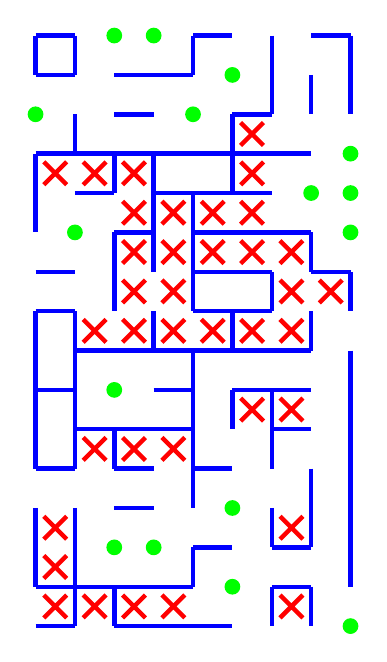
\begin{tikzpicture}[x=0.5cm, y=-0.5cm, ultra thick, blue]
% Walls
    \draw (0,0) -- (1,0);
    \draw (4,0) -- (5,0);
    \draw (7,0) -- (8,0);
    \draw (0,1) -- (1,1);
    \draw (2,1) -- (4,1);
    \draw (2,2) -- (3,2);
    \draw (5,2) -- (6,2);
    \draw (0,3) -- (7,3);
    \draw (1,4) -- (2,4);
    \draw (3,4) -- (6,4);
    \draw (2,5) -- (3,5);
    \draw (4,5) -- (7,5);
    \draw (0,6) -- (1,6);
    \draw (4,6) -- (6,6);
    \draw (7,6) -- (8,6);
    \draw (0,7) -- (1,7);
    \draw (4,7) -- (6,7);
    \draw (1,8) -- (7,8);
    \draw (0,9) -- (1,9);
    \draw (3,9) -- (4,9);
    \draw (5,9) -- (7,9);
    \draw (1,10) -- (4,10);
    \draw (6,10) -- (7,10);
    \draw (0,11) -- (1,11);
    \draw (2,11) -- (3,11);
    \draw (4,11) -- (5,11);
    \draw (2,12) -- (3,12);
    \draw (4,13) -- (5,13);
    \draw (6,13) -- (7,13);
    \draw (0,14) -- (4,14);
    \draw (6,14) -- (7,14);
    \draw (0,15) -- (1,15);
    \draw (2,15) -- (5,15);
    \draw (0,0) -- (0,1);
    \draw (0,3) -- (0,5);
    \draw (0,7) -- (0,11);
    \draw (0,12) -- (0,14);
    \draw (1,0) -- (1,1);
    \draw (1,2) -- (1,3);
    \draw (1,7) -- (1,11);
    \draw (1,12) -- (1,15);
    \draw (2,3) -- (2,4);
    \draw (2,5) -- (2,7);
    \draw (2,10) -- (2,11);
    \draw (2,14) -- (2,15);
    \draw (3,3) -- (3,6);
    \draw (3,7) -- (3,8);
    \draw (4,0) -- (4,1);
    \draw (4,4) -- (4,7);
    \draw (4,8) -- (4,12);
    \draw (4,13) -- (4,14);
    \draw (5,2) -- (5,4);
    \draw (5,7) -- (5,8);
    \draw (5,9) -- (5,10);
    \draw (6,0) -- (6,2);
    \draw (6,6) -- (6,7);
    \draw (6,9) -- (6,11);
    \draw (6,12) -- (6,13);
    \draw (6,14) -- (6,15);
    \draw (7,1) -- (7,2);
    \draw (7,5) -- (7,6);
    \draw (7,7) -- (7,8);
    \draw (7,11) -- (7,13);
    \draw (7,14) -- (7,15);
    \draw (8,0) -- (8,2);
    \draw (8,6) -- (8,7);
    \draw (8,8) -- (8,14);
% Pillars
    \fill[green] (2,0) circle(0.2);
    \fill[green] (3,0) circle(0.2);
    \fill[green] (5,1) circle(0.2);
    \fill[green] (0,2) circle(0.2);
    \fill[green] (4,2) circle(0.2);
    \fill[green] (8,3) circle(0.2);
    \fill[green] (7,4) circle(0.2);
    \fill[green] (8,4) circle(0.2);
    \fill[green] (1,5) circle(0.2);
    \fill[green] (8,5) circle(0.2);
    \fill[green] (2,9) circle(0.2);
    \fill[green] (5,12) circle(0.2);
    \fill[green] (2,13) circle(0.2);
    \fill[green] (3,13) circle(0.2);
    \fill[green] (5,14) circle(0.2);
    \fill[green] (8,15) circle(0.2);
% Inner points in accessible cul-de-sacs
    \node at (5.5,2.5) {};
    \node at (0.5,3.5) {};
    \node at (1.5,3.5) {};
    \node at (2.5,3.5) {};
    \node at (5.5,3.5) {};
    \node at (2.5,4.5) {};
    \node at (3.5,4.5) {};
    \node at (4.5,4.5) {};
    \node at (5.5,4.5) {};
    \node at (2.5,5.5) {};
    \node at (3.5,5.5) {};
    \node at (4.5,5.5) {};
    \node at (5.5,5.5) {};
    \node at (6.5,5.5) {};
    \node at (2.5,6.5) {};
    \node at (3.5,6.5) {};
    \node at (6.5,6.5) {};
    \node at (7.5,6.5) {};
    \node at (1.5,7.5) {};
    \node at (2.5,7.5) {};
    \node at (3.5,7.5) {};
    \node at (4.5,7.5) {};
    \node at (5.5,7.5) {};
    \node at (6.5,7.5) {};
    \node at (5.5,9.5) {};
    \node at (6.5,9.5) {};
    \node at (1.5,10.5) {};
    \node at (2.5,10.5) {};
    \node at (3.5,10.5) {};
    \node at (0.5,12.5) {};
    \node at (6.5,12.5) {};
    \node at (0.5,13.5) {};
    \node at (0.5,14.5) {};
    \node at (1.5,14.5) {};
    \node at (2.5,14.5) {};
    \node at (3.5,14.5) {};
    \node at (6.5,14.5) {};
% Entry-exit paths without intersections
\end{tikzpicture}
\end{center}
\vspace*{\fill}

\end{document}
